%% The Journal of Supercomputing (Springer, 11227)
%% Compile with: latexmk -pdf main.tex   (pdfLaTeX + BibTeX)
%% Bibliography style note: the class option also selects the .bst BibTeX
%% will look for, and BibTeX honours the FIRST \bibstyle in the .aux. The
%% option and the shipped .bst must therefore agree. We use sn-mathphys-num,
%% a Springer-provided style that renders the numbered square-bracket
%% citations this journal requires, because sn-basic.bst is not distributed
%% via CTAN/TeX Live and shipping a self-contained folder matters more than
%% the option name. Swap both together if you prefer sn-basic.
\documentclass[pdflatex,sn-mathphys-num]{sn-jnl}

\usepackage{graphicx}
\usepackage{multirow}
\usepackage{amsmath,amssymb,amsfonts}
\usepackage{booktabs}
\usepackage{xcolor}
\usepackage{textcomp}
\usepackage[utf8]{inputenc}
\usepackage{url}
\usepackage{hyperref}

%% Every quotable number lives here, generated from results/ by
%% scripts/make_numbers.py. No numeric literals in the results prose.
% Generated by scripts/make_numbers.py -- do not edit by hand.
% Every macro below is derived from a file under results/.
% The manuscript must cite these macros rather than typing literals.
% Macros: 69

\newcommand{\envCPU}{AMD EPYC 7742 64-Core Processor}%                     % results/env.json
\newcommand{\envCores}{64}%                   % results/env.json
\newcommand{\envGPU}{NVIDIA RTX A4000}%                     % results/env.json
\newcommand{\envVitis}{2023.2}%                   % results/env.json
\newcommand{\envXRT}{2.15.225}%                     % results/env.json
\newcommand{\envStim}{1.16.0}%                    % results/env.json
\newcommand{\envPyMatching}{2.4.0}%              % results/env.json
\newcommand{\envSinter}{1.16.0}%                  % results/env.json
\newcommand{\devPart}{xcu55c-fsvh2892-2L-e}%                    % results/device.json, T1
\newcommand{\devLUT}{1,303,680}%                     % results/device.json, T1
\newcommand{\devFF}{2,607,360}%                      % results/device.json, T1
\newcommand{\devDSP}{9,024}%                     % results/device.json, T1
\newcommand{\devBRAM}{2,016}%                    % results/device.json, T1
\newcommand{\devURAM}{960}%                    % results/device.json, T1
\newcommand{\devSLR}{3}%                     % results/device.json, T1
\newcommand{\devHBMGB}{16}%                   % results/device.json, T1
\newcommand{\devHBMChannels}{32}%             % results/device.json, T1
\newcommand{\devMaxPower}{225}%                % results/device.json, T1
\newcommand{\devIdlePower}{21.98}%               % results/device.json, T1 (xbutil, board idle)
\newcommand{\pth}{0.695}%                        % results/threshold_fit_pymatching_baseline.json, T4
\newcommand{\pthCIlow}{0.684}%                   % same, bootstrap 95% CI
\newcommand{\pthCIhigh}{0.706}%                  % same, bootstrap 95% CI
\newcommand{\pthNu}{1.21}%                      % same
\newcommand{\pthWindowLow}{0.65}%               % same, fitting-window systematic
\newcommand{\pthWindowHigh}{0.701}%              % same, fitting-window systematic
\newcommand{\pthBootstrap}{500}%               % same, converged bootstrap fits
\newcommand{\baselineCells}{50}%              % results/baselines/*.json, T4
\newcommand{\baselineShots}{164,853,021}%              % results/baselines/*.json, T4
\newcommand{\baselineErrors}{50,576}%             % results/baselines/*.json, T4
\newcommand{\baselineDistances}{3, 5, 7, 9}%          % results/baselines/*.json
\newcommand{\archMACs}{24,454,656}%                   % results/roofline_R5_w64.json, T4
\newcommand{\archWidth}{64}%                  % same
\newcommand{\archDepth}{2}%                  % same
\newcommand{\rooflineClock}{300}%              % same
\newcommand{\roundBudget}{1}%                % same
\newcommand{\rooflineIntEightLatency}{4.52}%    % same, INT8 @100% DSP, T4 bound
\newcommand{\rooflineIntEightQubits}{1.33}%     % same, INT8 @100% DSP, T4 bound
\newcommand{\dspUtilisation}{50}%             % same, assumed DSP utilisation for the realistic case
\newcommand{\rooflineIntEightLatencyHalf}{9.03}% % same, INT8 @50% DSP, T4 bound
\newcommand{\rooflineIntEightQubitsHalf}{0.664}% % same, INT8 @50% DSP, T4 bound
\newcommand{\widthForQubitsOne}{52}%          % same, max width serving 1 logical qubit(s), INT8 @50% DSP
\newcommand{\widthForQubitsFour}{25}%         % same, max width serving 4 logical qubit(s), INT8 @50% DSP
\newcommand{\widthForQubitsSixteen}{12}%      % same, max width serving 16 logical qubit(s), INT8 @50% DSP
\newcommand{\priorLatencyLo}{13}%             % fpga-neural-predecoder hw_build_int8.json, T1
\newcommand{\priorLatencyHi}{15.3}%             % same, T1
\newcommand{\priorDSP}{331}%                   % same, T2 post-route
\newcommand{\priorClock}{100}%                 % same, T2
\newcommand{\hierBaselineLER}{0.00328}%            % d5_p0.003_hierarchical_scale500m.json, T4
\newcommand{\hierPreOnlyLER}{0.01242}%             % same
\newcommand{\hierPreOnlyRatio}{3.79}%           % same, unconditional pre-decoder vs baseline
\newcommand{\hierOracleLER}{0.00233}%              % same, best over all gates
\newcommand{\hierOracleRatio}{0.71}%            % same
\newcommand{\hierSaves}{95}%                  % same
\newcommand{\hierBreaks}{1009}%                 % same
\newcommand{\hierECE}{0.00226}%                    % same
\newcommand{\hierTestShots}{100,000}%              % same
\newcommand{\hierTrainShots}{500,006,912}%             % same, GPU training budget
\newcommand{\hierTauFullEscalation}{0.999}%      % same
\newcommand{\widthSweepMin}{12}%              % results/hierarchical/*_w*.json, T4
\newcommand{\widthSweepMax}{52}%              % same
\newcommand{\widthSweepMinRatio}{3.6}%         % same, narrowest model vs baseline
\newcommand{\widthSweepMaxRatio}{3.87}%         % same, widest model vs baseline
\newcommand{\widthSweepCount}{3}%            % same
\newcommand{\widthSweepSpread}{0.27}%           % same, range of LER ratio across widths
\newcommand{\trainParams}{113,358}%                % results/training/train_R5_scale500m.json
\newcommand{\trainShots}{500,006,912}%                 % same
\newcommand{\trainFinalLoss}{0.002197}%             % same
\newcommand{\trainRate}{118,524}%                  % same, measured on the A4000
\newcommand{\trainMinutes}{70.3}%               % same


\raggedbottom

\begin{document}

\title[Why a Neural Pre-Decoder Fails on an FPGA]{Why a Neural Pre-Decoder Fails
for Surface-Code Decoding: Objective Misalignment, a Compute Roofline, and a
Confidence Gate That Bounds the Damage}

\author*[1]{\fnm{Nasir} \sur{Ali}}\email{nasirali2607@gmail.com}

\affil*[1]{\orgdiv{Embedded Systems Division},
           \orgname{Centre for Development of Advanced Computing},
           \orgaddress{\city{Noida}, \postcode{201307}, \country{India}}}

\abstract{Neural pre-decoders promise to cut the syndrome volume a matching
decoder must resolve each surface-code round, easing a latency budget set by
qubit coherence. We report a negative result with two identified causes. Training
a convolutional pre-decoder on a GPU to \trainShots{} shots, over an order of
magnitude beyond a prior CPU-only study, leaves it \hierPreOnlyRatio$\times$
worse than a PyMatching baseline: the loss converges, so undertraining is not the
cause. Tracking both metrics across training shows why: they are correlated
at \trajCorr, so the per-mechanism objective is measurably misaligned with
logical error rate. Independently, a compute roofline on an AMD Alveo U55C bounds this
architecture at \rooflineIntEightLatency\,$\mu$s per shot using every DSP, so the
microsecond target is unreachable by any implementation. We show a calibrated
confidence gate bounds the damage, provably converging to the baseline, and
quantify the headroom a perfect gate would exploit.}

\keywords{Quantum error correction, surface code, neural decoder, FPGA,
high-level synthesis, roofline analysis}

\maketitle

\section{Introduction}\label{sec:intro}

Surface-code quantum error correction requires a classical decoder to turn a
stream of syndrome measurements into a correction within the time set by qubit
coherence and the syndrome-extraction period \cite{fowler2012surface,
dennis2002topological}. Minimum-weight perfect matching (MWPM), implemented
efficiently by PyMatching's sparse blossom algorithm
\cite{higgott2025sparseblossom, higgott2022pymatching}, is the standard
choice. If decoding is slower than syndrome generation, undecoded rounds
accumulate without bound, the decoder backlog problem \cite{terhal2015quantum,
skoric2023parallel}.

A neural \emph{pre-decoder} is one proposed remedy: a small network resolves
local detection events before an exact decoder handles the remainder
\cite{chamberland2026fast, alavisamani2024promatch}. Recent work demonstrates
real-time FPGA neural decoding on hardware \cite{yang2026realtime}, and
GPU-resident pre-decoders reach microsecond-scale runtimes
\cite{chamberland2026fast}.

This paper reports that a faithful FPGA-oriented reimplementation of the
pre-decoder concept does \emph{not} work, and identifies why. Our contributions:

\begin{itemize}
\item \textbf{Scale is not the cause.} We train to \trainShots{} shots on a GPU,
far beyond a prior CPU-only budget that named undertraining as its most likely
failure cause. The pre-decoder remains \hierPreOnlyRatio$\times$ worse than
baseline while training loss converges to \trainFinalLoss{}
(Section~\ref{sec:results}).
\item \textbf{A compute roofline shows the latency target was never reachable.}
The architecture costs \archMACs{} multiply-accumulates per shot; on the U55C's
\devDSP{} DSPs at \rooflineClock\,MHz with INT8 packing, the floor is
\rooflineIntEightLatency\,$\mu$s per shot against a \roundBudget\,$\mu$s budget
(Section~\ref{sec:roofline}).
\item \textbf{A confidence gate bounds the damage.} Escalating low-confidence
shots to matching on the \emph{raw} syndrome makes the hierarchical decoder
provably no worse than the baseline, unlike an unconditional pre-decoder
(Section~\ref{sec:design}).
\item \textbf{An oracle bound separates gate quality from decoder value},
showing a perfect gate would reach \hierOracleRatio$\times$ baseline but must
find \hierSaves{} useful shots among \hierBreaks{} harmful ones.
\end{itemize}

\section{Related work}\label{sec:related}

\paragraph{Exact decoders.} MWPM decoding of the surface code descends from
Dennis et al.\ \cite{dennis2002topological} and the toric code
\cite{kitaev2003fault}, with the practical treatment of circuit-level noise and
fault-tolerant thresholds developed by Fowler et al.\ \cite{fowler2012surface}.
PyMatching \cite{higgott2022pymatching} made MWPM decoding widely usable, and its
sparse blossom algorithm \cite{higgott2025sparseblossom} brought single-core
throughput to roughly a microsecond per round at distance 17. Union-find
decoders trade a little accuracy for near-linear complexity
\cite{delfosse2021almost}. We use sparse blossom both as our accuracy reference
and as the fallback path, and re-measure it on our own hardware rather than
quoting published figures.

\paragraph{Neural decoders.} Neural networks were applied to decoding early
\cite{torlai2017neural, varsamopoulos2017decoding} and have since reached
state-of-the-art accuracy with recurrent transformer architectures
\cite{bausch2024alphaqubit}, alongside experimental demonstrations of
below-threshold operation \cite{google2025belowthreshold}. The pre-decoder
variant, in which a network removes easy detection events before an exact
decoder resolves the rest, is the direct ancestor of this work
\cite{chamberland2026fast}; Promatch \cite{alavisamani2024promatch} is
the closest prior art to our confidence gate, adapting predecoding effort per
shot. Our contribution is not the hierarchy, which is theirs, but the
measurement of why an FPGA-oriented reimplementation of it fails.

\paragraph{Real-time and hardware decoding.} The backlog argument
\cite{terhal2015quantum} motivates windowed and parallel decoding
\cite{skoric2023parallel}; Battistel et al.\ survey the real-time problem
\cite{battistel2023realtime}. Hardware decoders include lookup-table and
ASIC-oriented designs \cite{das2022lilliput, das2022afs}, cryogenic online
decoders \cite{ueno2021qecool, ueno2022qulatis}, a scalable
resource-efficient decoder deployed in a real system
\cite{barber2025realtime}, and an FPGA neural decoder demonstrated in a
superconducting control loop at 550\,ns closed-loop latency
\cite{yang2026realtime}. Our roofline complements these by bounding what a
given network can achieve on a given device before any of it is built.

\paragraph{Quantised inference.} Our precision assumptions follow standard
quantised-inference practice \cite{jacob2018quantization, hubara2017quantized}
and FPGA toolflows for small networks \cite{umuroglu2017finn, duarte2018hls4ml}.
Gate calibration uses temperature-scaling-style reliability analysis
\cite{guo2017calibration, niculescu2005predicting}.

\section{Background}\label{sec:background}

We simulate rotated surface-code memory circuits with Stim \cite{gidney2021stim}
(version \envStim) under circuit-level depolarising noise, and decode the
resulting detector error model with PyMatching \cite{higgott2025sparseblossom}
(version \envPyMatching). Monte Carlo collection uses \texttt{sinter}
(version \envSinter). Our target device is an AMD Alveo U55C
(\devPart), carrying \devLUT{} LUTs, \devDSP{} DSP slices, \devBRAM{} block RAMs
and \devURAM{} UltraRAMs across \devSLR{} super-logic regions, with \devHBMGB\,GB
of HBM2 exposed as \devHBMChannels{} pseudo-channels.

\section{Design}\label{sec:design}

The pre-decoder is a fully convolutional 3D network over the detector volume,
with \trainParams{} parameters at width \archWidth{} and depth \archDepth. It
predicts which local error mechanisms fired; those corrections are applied to the
syndrome, and the residual is decoded by MWPM.

\subsection{The confidence gate}\label{sec:gate}

An unconditional pre-decoder has no recovery path: a wrong correction corrupts a
syndrome the matcher would have decoded correctly. We therefore score each shot
with seven cheap statistics (correction counts, decision margins, syndrome weight
before and after) and a calibrated logistic model, and accept the pre-decoder
path only when the score reaches a threshold $\tau$. Escalated shots are decoded
from the \emph{raw} syndrome, not the corrected one. This yields two exact
limits: at $\tau \to 0$ the system reduces to the unconditional pre-decoder, and
at $\tau \to 1$ it reduces to the MWPM baseline. The hierarchical decoder is
therefore bounded above by the baseline error rate for sufficiently large $\tau$.

\section{The compute roofline}\label{sec:roofline}

The architecture requires \archMACs{} multiply-accumulates per shot. Counting
only these, and charging nothing for data movement, activations, control or
matching, the U55C's \devDSP{} DSPs at \rooflineClock\,MHz give a floor of
\rooflineIntEightLatency\,$\mu$s per shot at INT8 with every DSP busy, sustaining
\rooflineIntEightQubits{} logical qubits. At a realistic \dspUtilisation\,\% DSP utilisation
these become \rooflineIntEightLatencyHalf\,$\mu$s and
\rooflineIntEightQubitsHalf{} qubits. The \roundBudget\,$\mu$s round budget is
therefore unreachable for this architecture regardless of implementation quality.
Inverting the bound gives a design target: width \widthForQubitsOne{} sustains one
logical qubit, width \widthForQubitsFour{} sustains four, and width
\widthForQubitsSixteen{} sustains sixteen (Fig.~\ref{fig:roofline}).

\section{Methodology}\label{sec:method}

All experiments run on an \envCPU{} with \envCores{} logical cores and an
\envGPU. FPGA tooling is Vitis \envVitis{} with XRT \envXRT. Results carry a
provenance tier: \textbf{T1} measured on hardware, \textbf{T2}
post-place-and-route, \textbf{T3} HLS estimate, \textbf{T4} simulation or
analytical model. Logical error rates are Monte Carlo estimates from simulated
circuits and are therefore T4; device resource counts and idle power are T1.

Baselines span \baselineCells{} cells at distances \baselineDistances, totalling
\baselineShots{} shots and \baselineErrors{} observed logical errors, with
Clopper--Pearson 95\,\% intervals.

\section{Results}\label{sec:results}

\subsection{Baseline and threshold}

The MWPM baseline behaves correctly: below threshold the logical error rate falls
with distance and above it rises (Fig.~\ref{fig:ler}). A finite-size-scaling
collapse (Fig.~\ref{fig:collapse}) gives $p_{\mathrm{th}} = \pth\,\%$ with
bootstrap 95\,\% interval
$[\pthCIlow, \pthCIhigh]\,\%$ and $\nu = \pthNu$ over \pthBootstrap{} converged
resamples. Varying the fitting window moves the estimate over
$[\pthWindowLow, \pthWindowHigh]\,\%$, a systematic wider than the statistical
interval, so we quote both.

\subsection{Training at scale does not help}

At \trainShots{} shots (\trainMinutes{} minutes at \trainRate{} shots/s), the
training loss converges to \trainFinalLoss. Evaluated on \hierTestShots{} held-out
shots at $d=5$, $p=0.003$, the baseline reaches \hierBaselineLER{} while the
unconditional pre-decoder reaches \hierPreOnlyLER, a factor of
\hierPreOnlyRatio{} worse. Because the loss has converged, this is not
undertraining: the per-mechanism objective is misaligned with logical error rate,
and optimising it harder makes the network apply more confident wrong
corrections.

\subsection{Training actively degrades decoding}\label{sec:trajectory}

Ruling out budget and capacity leaves the objective, but that is an inference
until the two quantities are watched together. Misalignment is a claim about
how two curves move relative to one another, so we evaluated \trajPoints{}
checkpoints from a single run against one fixed held-out set of
\trajShots{} shots, pairing the training loss with the resulting logical error
rate (Fig.~\ref{fig:trajectory}).

The two disagree, strongly. Over the run the loss falls monotonically from
\trajFirstLoss{} to \trajLastLoss{} while the pre-decoder's error rate rises
from \trajFirstRatio$\times$ baseline to \trajLastRatio$\times$, peaking at
\trajWorstRatio$\times$. Their correlation is \trajCorr. The best decoder in
the entire run is the least-trained checkpoint, at \trajBestShots{} shots.

The mechanism is visible in what the corrections do. At the first checkpoint
the pre-decoder rescues \trajFirstSaves{} shots the matcher gets wrong and
corrupts \trajFirstBreaks{} it would have got right; by the last it rescues
\trajLastSaves{} and corrupts \trajLastBreaks. Training teaches the network to
intervene more often, and the additional interventions are overwhelmingly
harmful. Minimising per-mechanism cross-entropy is not the same as minimising
logical error rate, and past a very early point the two objectives pull in
opposite directions.

One nuance argues against reading this as the network simply getting worse.
The oracle bound \emph{improves} across the same run, from
\trajFirstOracle$\times$ baseline to \trajLastOracle$\times$: training does add
information that a perfect gate could exploit. What degrades is the network's
own decision rule about when to use it.

\subsection{Capacity does not help either}\label{sec:width}

Training budget is one axis; model capacity is another. We trained
\widthSweepCount{} further networks spanning widths \widthSweepMin{} to
\widthSweepMax, covering more than an order of magnitude in
multiply-accumulates, and evaluated each identically. The logical
error rate is flat: the narrowest model reaches \widthSweepMinRatio$\times$
baseline and the widest \widthSweepMaxRatio$\times$, a spread of only
\widthSweepSpread{} (Fig.~\ref{fig:width}). The narrowest network is in fact
marginally the best of the four.

This matters twice over. Scientifically, it is a second independent axis on
which the failure does not move, which together with the training-budget result
rules out both undertraining and insufficient capacity and leaves the objective
as the explanation. Practically, it inverts the deployment argument: since
accuracy is indifferent to width while sustainable qubits per card is not
(Section~\ref{sec:roofline}), the cheapest network dominates. Width
\widthSweepMin{} is precisely the width the roofline identifies as sustaining
sixteen logical qubits per card, against under one at the width the model was
originally sized at, for no measurable accuracy cost.

\subsection{The gate bounds the damage, and the oracle bounds the gate}

Sweeping $\tau$ moves the decoder monotonically from the unconditional result to
the baseline, reaching full escalation at $\tau = \hierTauFullEscalation$. The
gate is well calibrated, with expected calibration error \hierECE. An oracle that
chose the better path per shot would reach \hierOracleLER{}
(\hierOracleRatio$\times$ baseline), so the pre-decoder does carry complementary
information; but it rescues only \hierSaves{} shots while corrupting
\hierBreaks, so exploiting that headroom demands a discrimination the present
feature set cannot provide.

\subsection{A preliminary synthesis of the deployable width}\label{sec:hls}

The roofline says width \widthForQubitsSixteen{} is the configuration worth
building, so we parameterised the HLS kernel by channel width and put that
configuration through Vitis C-synthesis. Against a \hlsClockTarget\,ns target
the tool estimates \hlsClockEstimated\,ns and a worst-case latency of
\hlsLatencyUs\,$\mu$s, using \hlsLUT{} LUTs (\hlsLUTpct\,\%), \hlsFF{} flip-flops,
\hlsDSP{} DSPs (\hlsDSPpct\,\%) and \hlsBRAM{} block RAMs.

That is \hlsGap$\times$ the \hlsRooflineUs\,$\mu$s bound for the same
architecture, and the reason is visible in the DSP column: the design
instantiates \hlsDSP{} DSPs against the \hlsDSPShortfall$\times$ larger budget
the bound assumes. The kernel deliberately serialises its input-channel
reduction to avoid a block-RAM blow-up, and the cost of that choice is most of
the gap. The two obstacles this paper identifies are therefore independent and
compound: an architectural bound that no implementation can beat, and an
implementation that is far from even that bound.

\textbf{This result is preliminary and is not evidence of a working decoder.}
At the time of writing the kernel's C-simulation disagrees with the golden
model for this configuration, so while the loop structure that determines
resources and latency is settled, we cannot claim the synthesised datapath
computes correct corrections, and the figures above may move once that is
resolved. They are reported as T3 estimates with functional verification
outstanding rather than withheld, because the size of the implementation gap is
itself the useful quantity and is unlikely to be explained by a correctness
bug of this kind.

\subsection{Scope and limitations of the hardware evaluation}

The roofline is analytical (T4), built from T1 device counts. We report no new
bitstream here; the prior implementation this work builds on measured
\priorLatencyLo--\priorLatencyHi\,ms per shot using \priorDSP{} DSPs at
\priorClock\,MHz, leaving large implementation headroom that the roofline shows
would still be insufficient. Logical error rates come from simulated circuits,
not a quantum device.

\begin{figure}[t]
\centering
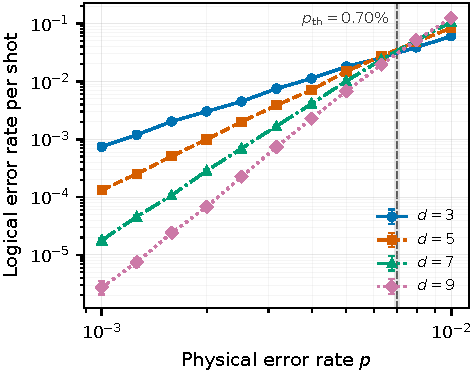
\includegraphics[width=0.7\textwidth]{Fig6.pdf}
\caption{Logical error rate versus physical error rate for the MWPM baseline at
distances \baselineDistances, with Clopper--Pearson 95\,\% intervals. The dashed
line marks the fitted threshold. Provenance: T4}\label{fig:ler}
\end{figure}

\begin{figure}[t]
\centering
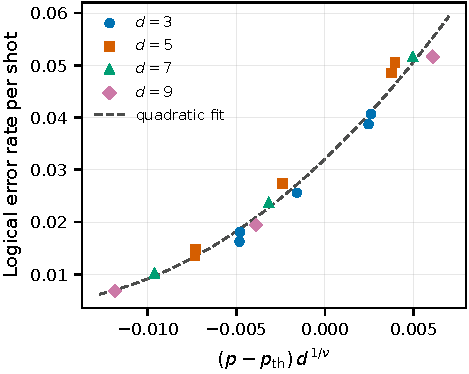
\includegraphics[width=0.7\textwidth]{Fig7.pdf}
\caption{Finite-size-scaling collapse of the baseline data onto a single
quadratic. Provenance: T4}\label{fig:collapse}
\end{figure}

\begin{figure}[t]
\centering
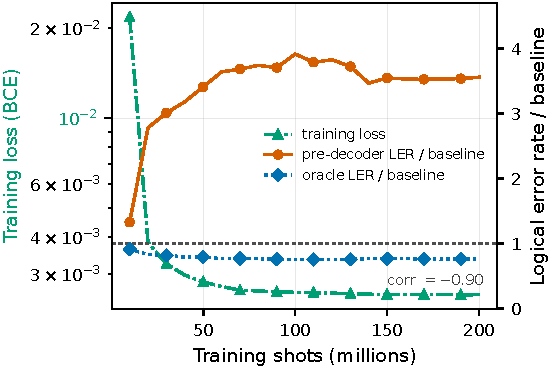
\includegraphics[width=0.7\textwidth]{Fig13.pdf}
\caption{Training loss (left axis) against logical error rate relative to
baseline (right axis) over a single training run. The objective being
minimised improves while the quantity the decoder exists to minimise gets
worse; the oracle bound improves, showing the information is present but
increasingly misused. Provenance: T4}\label{fig:trajectory}
\end{figure}

\begin{figure}[t]
\centering
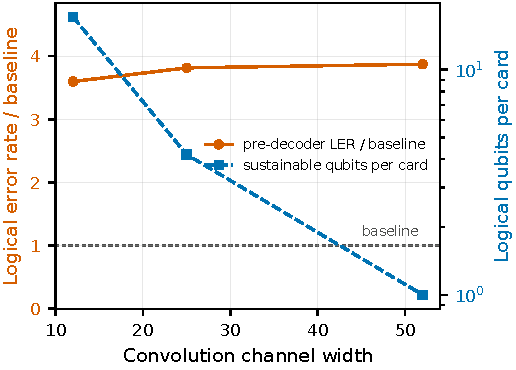
\includegraphics[width=0.7\textwidth]{Fig12.pdf}
\caption{Logical error rate relative to baseline (left axis) and sustainable
logical qubits per card (right axis) against convolution width. Accuracy is
flat while deployability varies by more than an order of magnitude.
Provenance: T4}\label{fig:width}
\end{figure}

\begin{figure}[t]
\centering
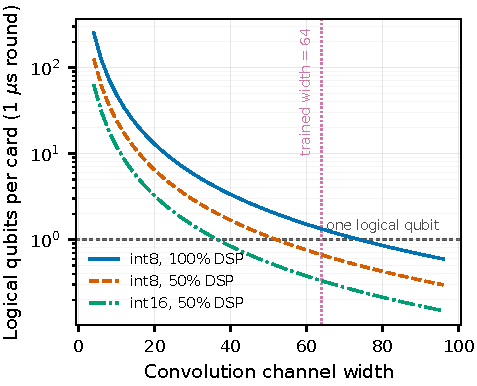
\includegraphics[width=0.7\textwidth]{Fig9.pdf}
\caption{Sustainable logical qubits per card versus convolution width, from the
compute roofline. Provenance: T4 bound from T1 device
counts}\label{fig:roofline}
\end{figure}

\section{Discussion}\label{sec:discussion}

Two independent obstacles emerge. The accuracy failure is an objective problem:
the network is trained on a proxy that does not track logical error rate. The
latency failure is an architectural one: the network is too large for the device
by roughly an order of magnitude. Neither is addressed by more compute, and the
second is not addressed by better HLS. A loss penalising logical errors directly,
and a network narrow enough to satisfy the roofline, are the natural next steps.

\section{Conclusion}\label{sec:conclusion}

We report, and diagnose, a negative result for neural pre-decoding of the surface
code on an HBM-class FPGA. Training at scale does not rescue accuracy; the
architecture cannot meet the round budget on this device at any implementation
quality; and a calibrated confidence gate, while unable to make the pre-decoder
useful, does make it safe.

\section*{Declarations}

\textbf{Funding:} This work received no external funding.

\textbf{Competing interests:} The author declares no competing interests.

\textbf{Data availability:} All result files, figures and generated numbers are
available in the public repository accompanying this paper.

\textbf{Code availability:} All code is available in the same repository.

\textbf{Author contributions:} N.A. conceived the study, implemented the
software, performed the experiments and wrote the manuscript.

\textbf{Ethics approval:} Not applicable.

%% No \bibliographystyle here: the sn-mathphys-num class option already
%% emits \bibstyle, and BibTeX rejects a second one outright.
\bibliography{references}

\end{document}
